\chapter{Introduction and Related Work}

%Replace \lipsum with text.
% You may have as many sections as you please. This is just for reference.

In this section, we will present the basic concepts necessary for understanding the Network virtualisation and the work that we will be presenting afterwards. We will start with concept of Virtualisation in general, subsequently moving onto the network virtualisation, software defined networking (SDN), virtual network management schemes in data centers and other related things.

\section{Virtualisation}
Virtualisation is the process of creating logical computing resources from available physical resources. It provides a layer of abstraction between workloads and the underlying physical hardware by means of virtualisation software. The virtualised computing resources such as CPUs, storage, network, disk I/O, memory are all pooled and provisioned to workloads without regard for physical location within a data centre.

It also provides encapsulation so that workload can access only the resources assigned to them. In this way several independent workloads can be supported in a virtualised system.

\subsection{Types of Virtualisation}
Various virtualisation technologies are as follows:-

\begin{itemize}
    \item \textbf{Server Virtualisation} - it abstracts the server physical computing resources from logical entities that are created. The user specifies the number of CPUs he requires and it is the virtualisation layer that maps it to the actual physical hardware. It increases the server utilisation.
    \item \textbf{Storage Virtualiastion} - it abstracts and pools the storage physical resources among workloads, thereby increasing storage utilisation. The user can specify the number and size of hard disk as part of parameters of it.
    \item \textbf{Network Virtualisation} - it allows to have multiple small logical network from large physical network and provision of large logical network from these multiple small networks. It helps network administrators to improve network traffic control, organisation and security.
\end{itemize}

\subsection{Benefits of Virtualisation}

There are several advantages of Virtualisation. Major ones are stated as:- 

\begin{itemize}
    \item \textbf{Save Expenditure}
     \item \textbf{Save Assets}
      \item \textbf{Improved Disaster Recovery}
       \item \textbf{Utilisation of Resources}
        \item \textbf{Centralisation of Management}
\end{itemize}


\section{Network Virtualisation}
The purpose of virtualisation is to simulate hardware services in software. All functionalities such as storage (in case of software defined storage) or network resources (in this case) are separated from the hardware and simulated in the software. The hardware platform can be any off the shelf general platform which allows for a more portable, scalable and cheaper solution.

When a network is virtualised, it creates a logical software-based view of the actual physical network and the functionalities of the network hardware boxes like routers, switches, etc. are implemented in the software itself. In this case physical device is only responsible for forwarding the packets, acting like a dumb switch, and all the routing and forwarding decisions are taken by the software.

Azodolmolky et. al. \cite{azodolmolky2013sdn} have studied different implementation of virtualization technologies and the table below summarizes the pro and cons of these technologies.

\begin{table}
\centering
\begin{tabular}{| p{6em} | p{5em} | p{1cm} | p{1cm} | p{5em} | p{5em} | p{5em} |}
\hline
{\bf Technology} & {\bf Bridging} & {\bf All host flooding } & {\bf vNet flooding} & {\bf VLAN 4k limit} & {\bf VM MAC visible} & {\bf State kept in network}\\ \hline
%
VLANs & Yes & Yes & Yes & Yes & Yes & Yes \\ \hline
%
VM-aware networking & Yes & No & Yes & Yes & Yes & Yes \\ \hline
vCDNI & Yes & Yes & Yes & No & No & MAC of hypervisors \\ \hline
VXLAN & No & Only to some hosts & Yes & No & No & Multicast groups \\ \hline
Nicira NVP & No & No & Some & No & No & No \\ \hline
\end{tabular}
\caption{Different network virtualization techniques}
\label{table:1}
\end{table}

\section{Software Defined Networking}
\subsection{Overview}
Software defined networking is referred to as the splitting of the network plane into a data plane and a control plane. The control plane consists solely the control logic and controls several devices in the data plane. The data plane, on the other hand, solely consists of forwarding logic such as switches. The control plane is considered to be dumb as it just forwards packets based on the instructions given by the control plane.

\subsection{Need for SDN}
Software defined networking is a framework which allows network programmers to automatically manage and control a large number of network devices, services, topology, traffic paths using high level languages and APIs. SDN pulls out the abstractions and allows one to look at the bigger picture. 
\begin{itemize}
    \item Virtualization: Use of network resources without worrying about where it is physically located.
    \item Orchestration: Ability to control and manage thousands of devices with a few commands.
    \item Programmable: Ability to change behaviour dynamically without the need to suspend services.
    \item Visibiltiy: It allows the monitoring of resources and figure is the network is disrupted or the presence of any faults.
    \item Performance: It also allows traffic engineering (bandwidth management), load balancing, high utilization and error handling.
    \item Multi-tenancy: The tenants have a complete control over their addresses, topology, routing and security.
\end{itemize}

\begin{figure}[h]
\begin{center}	
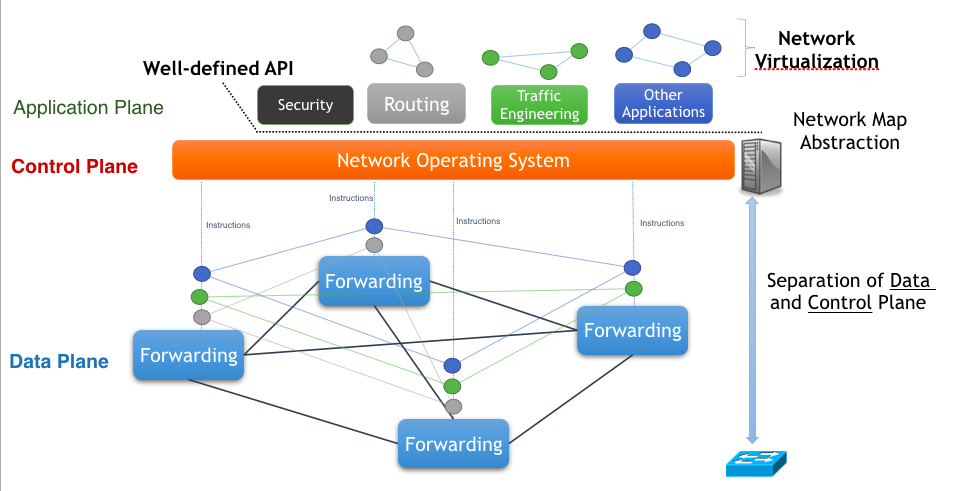
\includegraphics[scale=0.4]{data_control_plane} 
\caption{Separation of data and control planes }
\label{fig:data_control_plane}
\end{center}
\end{figure}

\subsection{Data and Control planes}
SDN consists of two separate planes which are data plane and control plane. In the traditional network where the forwarding logic is distributed to in the network. One example of this type of distribution is in the linked state routers where routers exchange information with each other to jointly create and image of the network while none of them have the complete view of the network. Unlike the traditional network, in SDN, the network intelligence is and states are logically abstracted out. The underlying network infrastructure is abstracted out from applications.
\begin{itemize}
    \item Data plane: The forwarding logic like switches run of general purpose commodity hardware. It is decoupled from specific networking hardware
    \item Control plane: The data plane is controlled, maintained and programmed from a central entity called a control plane 
\end{itemize}

\begin{figure}[h]
\begin{center}	
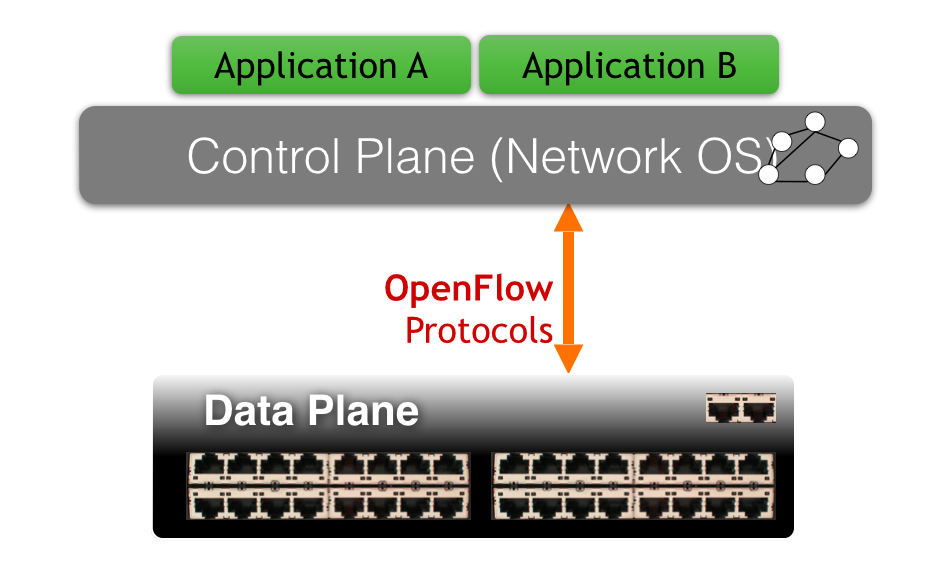
\includegraphics[scale=0.4]{openflow} 
\caption{OpenFlow}
\label{fig:openflow}
\end{center}
\end{figure}

\subsection{OpenFlow}
OpenFlow is a software defined networking standard which allows network controllers to determine the path of network packets across a network of switches. It is a communication interface between the control plane and data plane of an SDN architecture. It allows direct access to and manipulation of the forwarding plane of network devices such as switches and routers, both physical and virtual. It can also be thought as a protocol used in switching devices and controllers interface.

\subsubsection{Working of OpenFlow}
OpenFlow manages the traffic (network flows) by manipulating a flow table at switches. Instructions are stored in flow tables. When a packet arrives at a switch, it matches the header fields with flow entries in a flow table. If any entry is matched, it performs indicated actions and updates the counters. If, however, it is not matches then the switch asks the controller by sending a message with the packet header.

\subsubsection{OpenFlow table}
The basic actions in an OpenFlow table are as follows:
\begin{itemize}
    \item All: To all interfaces except the incoming interface.
    \item Controller: Encapsulate the packet and send it to the controller.
    \item Local: Send to its local networking stack
    \item Table: Perform actions in the next flow table 
    \item In\_port: Send the packet back to the input port.
    \item Normal: Forward in accordance with the traditional ethernet.
    \item Flood: Send along the minimum spanning tree except the incoming interface.
\end{itemize}


\section{Baadal: IIT Delhi's Private Cloud}

\section{Related Work}

\subsection{Data Center architectures}

\subsection{Online traffic aware virtual machine placement in data center networks}
Dias et. al.\cite{dias2012online} have presented a virtual machine placement (VMP) algorithm to reallocate virtual machines in the data center servers based on the current traffic matrix, CPU, and memory usage. VMP takes into account the current data center work load, CPU and memory usage of virtual machines to avoid bottlenecks. The basic idea is to consolidate virtual machines that have correlated services. VMP operation is divided into four parts:

\begin{itemize}
    \item Data acquisition: The traffic between each pair of virtual machines is used to create a traffic matrix. It also takes the CPU and memory usage of each virtual machine as input as well as the topology of the data center. The most used topologies used are similar as all of them have a core which is responsible for connecting big segments of the network. Traffic engineering tries to push the traffic to the edges of the network thereby reducing it in the higher layers. 
    \item Server partitioning: They also have proposed an algorithm for partitioning of servers. The servers which have high degree of connectivity are clubbed together. Most suitable candidates for this type of aggregation are the servers which are placed at the same layers.
    \item Clustering virtual machines: They \cite{dias2012online} have used a community finding algorithm to find communities withing the virtual machines which clusters the virtual machines into groups which have high degree of connectivity.
    \item VM assignment: In the final step the virtual machines (which are clustered into communities by now) are allocated server partitions which were obtained in the server partitioning step.
\end{itemize}
In the simulations they have shown that their method is scalable to big data centers and provides an improvement of 12.5\% over no management.

\subsection{Traffic Engineering}
Jiang et. al. \cite{jiang2012joint} have proposed a solution to the problem of network load balancing by means of a joint tenant placement and route selection by exploiting multipath routing capability and dynamic virtual machine migration. They have proposed an offline algorithm that solves a static problem given a network snapshot, and an online solution for a dynamic environment with changing traffic. They have leveraged the technique of Markov approximation what required a very small number of virtual machine migrations. In simulations done by them they have evaluated the performance of online algorithms with real workload obtained from large computing clusters and have shown that their algorithm incurs the minimum performance cost in comparison to all other tested algorithms.

Biran et. al. \cite{biran2012stable} have also studied this problem and said that VM placement has to carefully consider the aggregate resource consumption of co-located VMs in order to obey service level agreements at lower possible cost. Also, the traffic patterns are not stable in nature and vary over a period of time. They have addressed this problem by trying to allocate a placement that not only satisfies the predicted communication demand but also is resilient to demand time-variations. They have defined the problem as a min cut ratio-aware VM placement which is NP-hard in general but they have employed several heuristics to solve it. Through their simulations they have shown that the placements based on their algorithm increase data scalability, while being able to support time-varying traffic demands with a reduced number of dropped packets. 